\section{Date: 2026-09-20}
\noindent \textbf{Series ID: CBR01127ALA647NCEN} 

\noindent This series is titled SNAP Benefits Recipients in Walker County, AL and has a frequency of Annual. The units are Persons and the seasonal adjustment is Not Seasonally Adjusted.The observation start date is 1989-01-01 and the observation end date is 2023-01-01.The popularity of this series is 1. \\ 

\noindent \textbf{Series ID: SLRTTO02EEA661S} 

\noindent This series is titled Sales: Retail Trade: Total Retail Trade: Value for Estonia and has a frequency of Annual. The units are Index 2015=100 and the seasonal adjustment is Seasonally Adjusted.The observation start date is 1995-01-01 and the observation end date is 2022-01-01.The popularity of this series is 1. \\ 

\subsection{Raw Regression}
\noindent Regresses the two series against each other directly. A significant result here can come just as easily from both series sharing a long-run trend as from any real relationship.

\begin{center}
\begin{tabular}{lclc}
\toprule
\textbf{Dep. Variable:}                  & value\_fred\_SLRTTO02EEA661S & \textbf{  R-squared:         } &     0.504   \\
\textbf{Model:}                          &             OLS              & \textbf{  Adj. R-squared:    } &     0.484   \\
\textbf{Method:}                         &        Least Squares         & \textbf{  F-statistic:       } &     25.41   \\
\textbf{Date:}                           &       Sun, 20 Sep 2026       & \textbf{  Prob (F-statistic):} &  3.36e-05   \\
\textbf{Time:}                           &           14:58:36           & \textbf{  Log-Likelihood:    } &   -128.52   \\
\textbf{No. Observations:}               &                27            & \textbf{  AIC:               } &     261.0   \\
\textbf{Df Residuals:}                   &                25            & \textbf{  BIC:               } &     263.6   \\
\textbf{Df Model:}                       &                 1            & \textbf{                     } &             \\
\textbf{Covariance Type:}                &          nonrobust           & \textbf{                     } &             \\
\bottomrule
\end{tabular}
\begin{tabular}{lcccccc}
                                         & \textbf{coef} & \textbf{std err} & \textbf{t} & \textbf{P$> |$t$|$} & \textbf{[0.025} & \textbf{0.975]}  \\
\midrule
\textbf{const}                           &      -1.7917  &       16.658     &    -0.108  &         0.915        &      -36.100    &       32.517     \\
\textbf{value\_fred\_CBR01127ALA647NCEN} &       0.0090  &        0.002     &     5.040  &         0.000        &        0.005    &        0.013     \\
\bottomrule
\end{tabular}
\begin{tabular}{lclc}
\textbf{Omnibus:}       &  7.952 & \textbf{  Durbin-Watson:     } &    0.179  \\
\textbf{Prob(Omnibus):} &  0.019 & \textbf{  Jarque-Bera (JB):  } &    6.195  \\
\textbf{Skew:}          &  1.112 & \textbf{  Prob(JB):          } &   0.0452  \\
\textbf{Kurtosis:}      &  3.748 & \textbf{  Cond. No.          } & 2.74e+04  \\
\bottomrule
\end{tabular}
%\caption{OLS Regression Results}
\end{center}

Notes: \newline
 [1] Standard Errors assume that the covariance matrix of the errors is correctly specified. \newline
 [2] The condition number is large, 2.74e+04. This might indicate that there are \newline
 strong multicollinearity or other numerical problems.

\begin{figure}
\centering
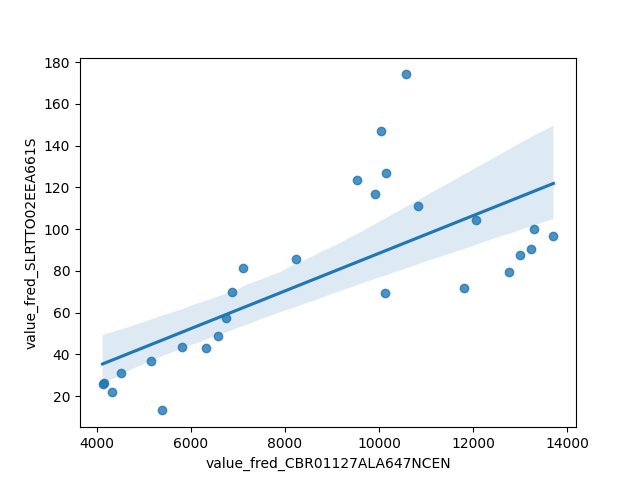
\includegraphics[scale = 0.9]{plots/plot_2026-09-20.png}
\caption{Raw Regression Plot for 2026-09-20}
\end{figure}
\newpage
\subsection{Detrended Regression}
\noindent Regresses the residuals of each series after removing its own linear time trend, so a shared trend can no longer drive the result on its own. A relationship that stays significant here is better evidence of a genuine link between the two series.

\begin{center}
\begin{tabular}{lclc}
\toprule
\textbf{Dep. Variable:}                             & value\_fred\_SLRTTO02EEA661S\_detrended & \textbf{  R-squared:         } &     0.247   \\
\textbf{Model:}                                     &                   OLS                   & \textbf{  Adj. R-squared:    } &     0.217   \\
\textbf{Method:}                                    &              Least Squares              & \textbf{  F-statistic:       } &     8.214   \\
\textbf{Date:}                                      &             Sun, 20 Sep 2026            & \textbf{  Prob (F-statistic):} &  0.00831    \\
\textbf{Time:}                                      &                 14:58:36                & \textbf{  Log-Likelihood:    } &   -93.880   \\
\textbf{No. Observations:}                          &                      27                 & \textbf{  AIC:               } &     191.8   \\
\textbf{Df Residuals:}                              &                      25                 & \textbf{  BIC:               } &     194.4   \\
\textbf{Df Model:}                                  &                       1                 & \textbf{                     } &             \\
\textbf{Covariance Type:}                           &                nonrobust                & \textbf{                     } &             \\
\bottomrule
\end{tabular}
\begin{tabular}{lcccccc}
                                                    & \textbf{coef} & \textbf{std err} & \textbf{t} & \textbf{P$> |$t$|$} & \textbf{[0.025} & \textbf{0.975]}  \\
\midrule
\textbf{const}                                      &    1.344e-12  &        1.566     &  8.58e-13  &         1.000        &       -3.226    &        3.226     \\
\textbf{value\_fred\_CBR01127ALA647NCEN\_detrended} &      -0.0024  &        0.001     &    -2.866  &         0.008        &       -0.004    &       -0.001     \\
\bottomrule
\end{tabular}
\begin{tabular}{lclc}
\textbf{Omnibus:}       & 15.687 & \textbf{  Durbin-Watson:     } &    0.784  \\
\textbf{Prob(Omnibus):} &  0.000 & \textbf{  Jarque-Bera (JB):  } &   17.422  \\
\textbf{Skew:}          &  1.448 & \textbf{  Prob(JB):          } & 0.000165  \\
\textbf{Kurtosis:}      &  5.664 & \textbf{  Cond. No.          } & 1.90e+03  \\
\bottomrule
\end{tabular}
%\caption{OLS Regression Results}
\end{center}

Notes: \newline
 [1] Standard Errors assume that the covariance matrix of the errors is correctly specified. \newline
 [2] The condition number is large, 1.9e+03. This might indicate that there are \newline
 strong multicollinearity or other numerical problems.

\begin{figure}
\centering
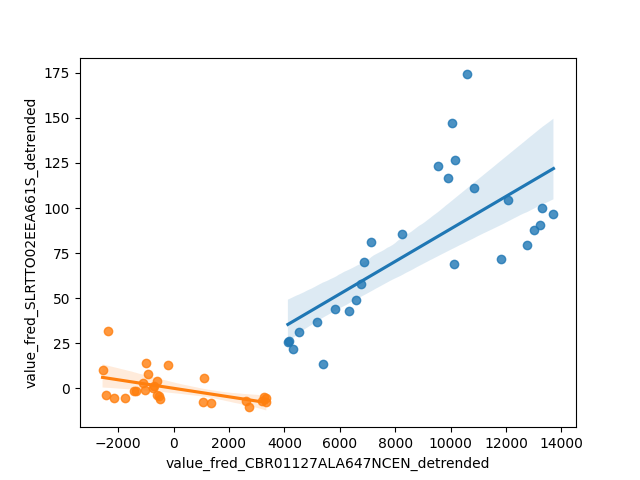
\includegraphics[scale = 0.9]{plots/plot_2026-09-20_detrended.png}
\caption{Detrended Regression Plot for 2026-09-20}
\end{figure}
\newpage
